\ifdefined\handout
  \documentclass[handout]{beamer}
\else
  \documentclass{beamer}
\fi

\usetheme{boxes}
\usecolortheme{structure}

\setbeamertemplate{footline}[frame number]

\ifdefined\handout
\definecolor{beamer@structure@color}{rgb}{0,0,0}
\setbeamertemplate{navigation symbols}{}
\setbeamercolor{normal text}{fg=black,bg=white}
\setbeamertemplate{frametitle}{\vskip 15pt\color{black}
\def\myhrulefill{\leavevmode\leaders\hrule height 1pt\hfill\kern 0pt}
\headingfont\insertframetitle\par\vskip-8pt\myhrulefill}
\else
\definecolor{beamer@structure@color}{rgb}{1,1,1}
\setbeamertemplate{navigation symbols}{}
\setbeamercolor{normal text}{fg=white,bg=black}
\setbeamertemplate{frametitle}{\vskip 15pt\color{white}
\def\myhrulefill{\leavevmode\leaders\hrule height 1pt\hfill\kern 0pt}
\headingfont\insertframetitle\par\vskip-8pt\myhrulefill}
\fi

\usepackage{amsmath,amssymb}

\newcommand{\NN}{\mathbb{N}}
\newcommand{\ZZ}{\mathbb{Z}}

\DeclareMathOperator{\mcd}{mcd}
\DeclareMathOperator{\mcm}{mcm}

\usepackage[spanish]{babel}

\usepackage{tikz-cd}
\usetikzlibrary{babel}
\usetikzlibrary{calc}

\usepackage{framed}

\newcommand{\dfn}{\mathrel{\mathop:}=}
\newcommand{\rdfn}{=\mathrel{\mathop:}}

\usepackage{mathspec}
\setsansfont[BoldFont={IBM Plex Sans Bold}, ItalicFont={IBM Plex Sans Italic}]{IBM Plex Sans}
\setmonofont[BoldFont={IBM Plex Mono Bold}, ItalicFont={IBM Plex Mono Italic}]{IBM Plex Mono}
\setmathrm[BoldFont={IBM Plex Sans Bold}, ItalicFont={IBM Plex Sans Italic}]{IBM Plex Sans}
\newfontfamily\headingfont[]{IBM Plex Sans Bold}

\setbeamercovered{transparent=10}


\begin{document}

\begin{frame}[plain,noframenumbering]
  \textbf{INTRODUCCIÓN A LA TEORÍA DE NÚMEROS}

  Alexey Beshenov $\mid$ \texttt{cadadr.org}

  \vfill

  \begin{center}\huge\headingfont
    DIVISIÓN CON RESIDUO (EUCLIDIANA)
  \end{center}

  \vfill
\end{frame}

\begin{frame}
  \frametitle{¿DE QUÉ SE TRATA?}

  \begin{itemize}
  \item<2-> $20$ es divisible por
    $1$, $2$, $4$, $5$, $10$, $20$.

  \item<3-> $20$ no es divisible por $3$, pero podemos escribir
    \[ \frac{20}{3} = 6\,\frac{2}{3}. \]

  \item<4-> \textbf{División con residuo} (= \textbf{división euclidiana}):
    \[ 20 = 6\cdot 3 + 2. \]
    \onslide<5->{$6$ es el \textbf{cociente} y $2$ es el \textbf{residuo} de división por $3$.}
  \end{itemize}
\end{frame}

\begin{frame}
  \frametitle{DIVISIÓN CON RESIDUO (EUCLIDES)}

  \begin{minipage}[t][0.6\textheight]{0.6\textwidth}
    \onslide<2->{\vspace{0pt}
      Para cualesquiera dos enteros $a$ y ${b \ne 0}$, existen enteros
      $q$ (\textbf{cociente}) y $r$ (\textbf{residuo}) tales que

      \[ a = qb + r,
        \quad
        0 \le r < |b|. \]}

    \onslide<3->{Además, estos $q$ y $r$ están definidos de manera única.}
  \end{minipage}
  \begin{minipage}[t]{0.35\textwidth}
    \vspace{0pt}\flushright
    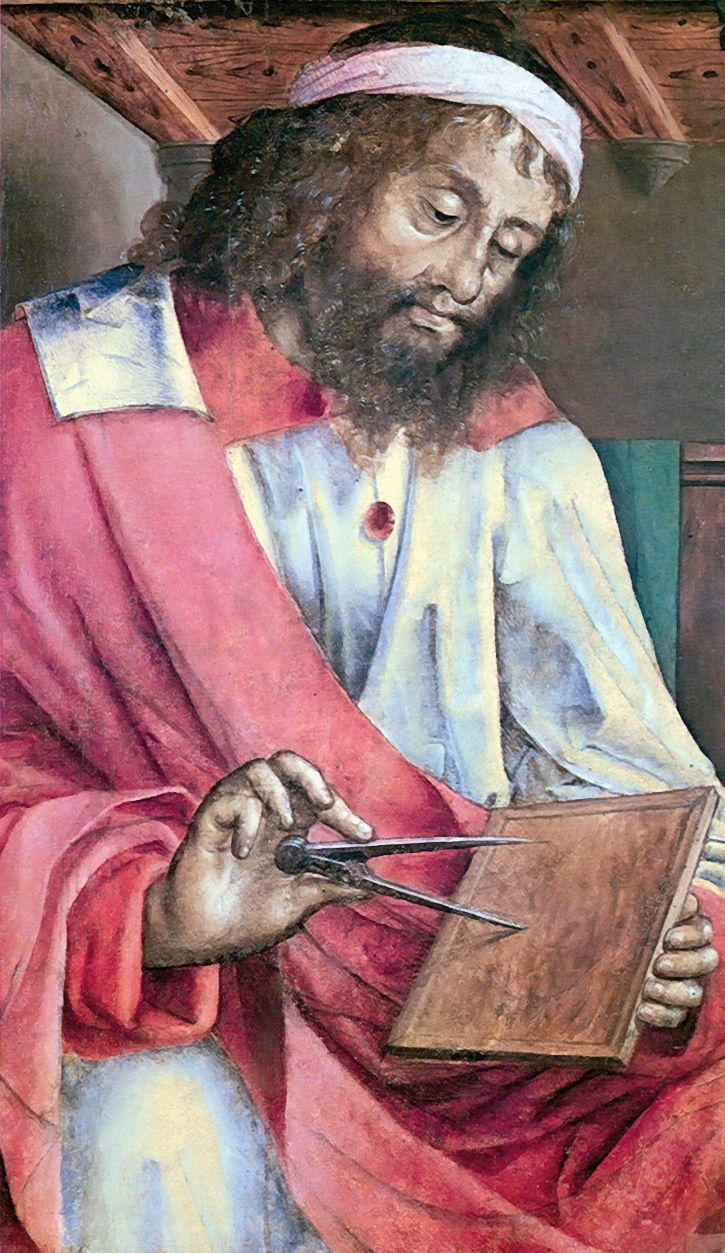
\includegraphics[width=.9\textwidth]{euclides.jpg}
    Euclides \\
    (ca. 325--265 a.C.)
  \end{minipage}
\end{frame}

\begin{frame}
  \frametitle{PRIMERA DEMOSTRACIÓN DE EXISTENCIA}

  \begin{framed}
      \[ a = qb + r,
        \quad
        0 \le r < |b|. \]
    \end{framed}

  \onslide<2->{
    \[ q \dfn
      \begin{cases}
        \lfloor a/b\rfloor, & \text{si }b > 0,\\
        \lceil  a/b\rceil,  & \text{si }b < 0,
      \end{cases} \]}
  \onslide<3->{donde
    \begin{align*}
      \lfloor x \rfloor & \dfn \max \{ n \in \ZZ \mid n \le x \}, \\
      \lceil x \rceil & \dfn \min \{ n \in \ZZ \mid n \ge x \}.
    \end{align*}}
    \onslide<4->{Para $r = a - qb$ se cumple $0 \le r < |b|$. \qed}

  \vspace{\fill}
\end{frame}

\begin{frame}
  \frametitle{SEGUNDA DEMOSTRACIÓN DE EXISTENCIA}

  \begin{framed}
    \[ a = qb + r,
      \quad
      0 \le r < |b|. \]
  \end{framed}

  \onslide<2->{Consideremos el conjunto
    $$X = \{ a - qb \mid q \in \ZZ \}.$$}

  \onslide<3->{Sea $r = a - qb \ge 0$ el mínimo elemento no negativo de $X$.}

  \onslide<4->{Entonces, $a = qb + r$ es la expresión deseada. \qed}

  \vspace{\fill}
\end{frame}

\begin{frame}
  \frametitle{DEMOSTRACIÓN DE UNICIDAD}

  \begin{framed}
    \[ a = qb + r,
      \quad
      0 \le r < |b|. \]
  \end{framed}

  \begin{itemize}
  \item<2-> Supongamos que
    $a = qb + r = q' b + r'$,

    donde $0 \le r, r' < |b|$.

  \item<3-> Sin pérdida de generalidad, $r' \ge r$.
    $$0 = (q'-q)\,b + (r'-r) \iff r' - r = (q-q')\,b.$$

  \item<4-> $b \mid (r' - r)$, pero $0 \le r' - r < |b|$.

    Entonces, $r = r'$ y $q = q'$. \qed
  \end{itemize}

  \vspace{\fill}
\end{frame}

\begin{frame}
  \frametitle{EJEMPLOS}

  \begin{itemize}
  \item<2-> $b \mid a$ si y solamente si $r = 0$ y $q = a/b$

    (la división es posible sin residuo).

  \item<3-> El residuo de división por $b = 2$ es

    \begin{itemize}
    \item<4-> $r = 0$, cuando $a = 2n$ es un \textbf{número par};
    \item<5-> $r = 1$ cuando $a = 2n+1$ es un \textbf{número impar}.
    \end{itemize}

  \item<6-> Para $a = 117$ y $b = 7$ la calculadora sugiere que
    $\frac{117}{7} = 16.714285\ldots$

    \onslide<7->{Tomamos $q = 16$, $r = a - qb = 5$.}

    \onslide<8->{$117 = 16\cdot 7 + 5 \iff (q,r) = (16,5)$.}
  \end{itemize}
\end{frame}

\begin{frame}
  \frametitle{APLICACIÓN CURIOSA}

  \begin{itemize}
  \item<2-> $a = 15131$ no es un \textbf{cuadrado entero}:
    no existe $b \in \ZZ$ tal que $a = b^2$.

  \item<3-> De hecho, $\sqrt{a} = 123.008129\ldots$

  \item<4-> Una prueba aritmética: dividiendo con residuo por $3$,
    $$a = 5043 \cdot 3 + 2.$$

  \item<5-> Si $b = 3n + r$ con $r \in \{ 0, 1, 2 \}$, entonces
    \[
      b^2 = \underbrace{9\,n^2 + 6\,nr}_{\text{divisible por }3} + r^2,
      \quad
      r^2 = 0, 1, 4.
    \]
    $b^2$ debe dar residuo $0$ o $1$ de división por $3$.

  \item<6-> Conclusión: $a \ne b^2$. \qed
  \end{itemize}
\end{frame}

\begin{frame}
  \frametitle{EJERCICIO}

  \onslide<2->{\begin{framed}
      Use la misma idea para probar que $2022$ no es un cubo

      (es decir, $2022 \ne b^3$ para $b \in \ZZ$).
    \end{framed}}

  \onslide<3->{Sugerencia: divida $2022$ por $4$;

    ¿qué residuo de división por $4$ puede tener $b^3$?}
\end{frame}

\begin{frame}
  \frametitle{* PROGRESIONES GEOMÉTRICAS}

  \onslide<2->{\begin{framed}
      $$1 + x + x^2 + \cdots + x^{q-1} = \frac{x^q - 1}{x - 1}.$$
    \end{framed}}
  \onslide<3->{\emph{Demostración}:
    \begin{multline*}
      (1 + x + \cdots + x^{q-2} + x^{q-1})\,(x-1) = \\
      (x + x^2 + \cdots + x^{q-1} + x^q) -
      (1 + x + \cdots + x^{q-2} + x^{q-1}) = \\
      x^q - 1. \qed
    \end{multline*}}
\end{frame}

\begin{frame}
  \frametitle{COROLARIO}
  \onslide<2->{\begin{framed}
      Para $a > 1$ y $m,n \ge 0$, si $m \mid n$, entonces
      $(a^m - 1) \mid (a^n - 1)$.
    \end{framed}}

  \onslide<3->{\emph{Demostración}:
    \begin{equation*}
      \frac{a^n - 1}{a^m - 1} = \frac{(a^m)^{n/m} - 1}{a^m - 1} =
      1 + a^m + a^{2m} + \cdots + (a^m)^{n/m-1} \in \ZZ. \qed
    \end{equation*}}

  \onslide<4->{\textbf{Ejemplo}:
    $65535 = 2^{16} - 1$ es divisible por $15 = 2^4 - 1$:
    $$65535 = 4369\cdot 15.$$}

  \onslide<5->{¿Es cierto que $a^m - 1 \mid a^n - 1$ implica que
    $m \mid n$?}
\end{frame}

\begin{frame}
  \frametitle{OTRA APLICACIÓN CURIOSA}
  \begin{framed}
    Para $a > 1$ y $m, n \ge 0$, se tiene
    $$(a^m - 1) \mid (a^n-1) \iff m \mid n.$$
  \end{framed}

  \onslide<2->{Dividamos con residuo $n = qm + r$.}

  \begin{align*}
    \onslide<3->{\frac{a^n-1}{a^m-1}} & \onslide<3->{= \frac{(a^{qm + r} - a^r) + (a^r - 1)}{a^m - 1}} \\
                        & \onslide<4->{= \frac{a^{qm} - 1}{a^m - 1}\,a^r + \frac{a^r - 1}{a^m - 1}} \\
                        & \onslide<5->{= \underbrace{a^r \, \sum_{0 \le i < q} a^{im}}_{\text{entero}} + \frac{a^r - 1}{a^m - 1}.}
  \end{align*}
\end{frame}

\begin{frame}
  \frametitle{OTRA APLICACIÓN CURIOSA (CONT.)}
  \begin{framed}
    $$(a^m - 1) \mid (a^n-1) \iff m \mid n.$$
  \end{framed}
  \onslide<2->{\[ \frac{a^n-1}{a^m-1} = \underbrace{a^r \, \sum_{0 \le i < q} a^{im}}_{\text{entero}} + \frac{a^r - 1}{a^m - 1}. \]}
  \onslide<3->{$$(a^m - 1) \mid (a^n-1) \iff (a^m - 1) \mid (a^r - 1) \iff r = 0 \iff m \mid n,$$
  Usando que $0 \le r < m$. \qed}
\end{frame}

\begin{frame}
  \frametitle{EJERCICIO: PRIMOS DE MERSENNE}

  \onslide<2->{\begin{framed}
      Si un número de la forma $a^p - 1$ es primo, entonces necesariamente $a = 2$
      y $p$ es primo.
    \end{framed}}

  \begin{itemize}
  \item<3-> \textbf{Ejemplo}:
    \onslide<4->{$2^5 - 1 = 31$ es primo.} \\
    \onslide<5->{$2^6 - 1 = 63 = 7\cdot 9$ no es primo.} \\
    \onslide<6->{$6^5 - 1 = 7775 = 25\cdot 311$ no es primo.}

  \item<7-> ¡No todos los $2^p - 1$ son primos!

    \onslide<8->{Primer contraejemplo: $2^{11} - 1 = 2047 = 23\cdot 89$.}

  \item<9-> Los primos de la forma $2^p - 1$ se llaman los

    \textbf{primos de Mersenne}.
  \end{itemize}
\end{frame}

\begin{frame}
  \frametitle{PRIMOS DE MERSENNE}

  \begin{minipage}[t][0.6\textheight]{0.6\textwidth}
    \vspace{-20pt}
    \begin{align*}
      \onslide<2->{2^2 - 1} & \onslide<2->{= 3,} \\
      \onslide<3->{2^3 - 1} & \onslide<3->{= 7,} \\
      \onslide<4->{2^5 - 1} & \onslide<4->{= 31,} \\
      \onslide<5->{2^7 - 1} & \onslide<5->{= 127,} \\
      \onslide<6->{2^{11} - 1} & \onslide<6->{= 23\cdot 89,} \\
      \onslide<7->{2^{13} - 1} & \onslide<7->{= 8191,} \\
      \onslide<8->{2^{17} - 1} & \onslide<8->{= 131071,} \\
      \onslide<9->{2^{19} - 1} & \onslide<9->{= 524287,} \\
      \onslide<10->{2^{23} - 1} & \onslide<10->{= 47\cdot 178481,} \\
      & \onslide<11->{\cdots}
    \end{align*}
  \end{minipage}
  \begin{minipage}[t]{0.35\textwidth}
    \vspace{0pt}\flushright
    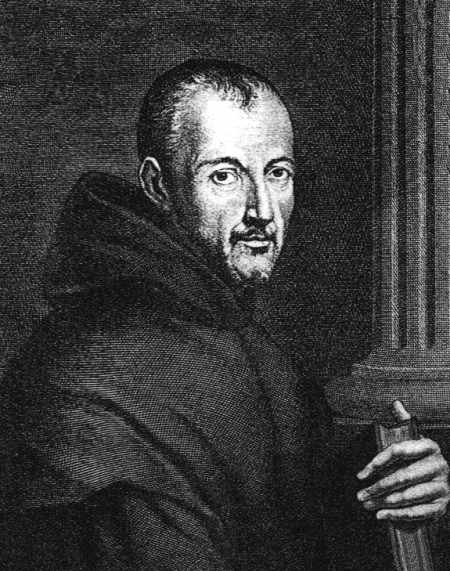
\includegraphics[width=.9\textwidth]{mersenne.jpg}

    Marin Mersenne\\
    (1588--1648)
  \end{minipage}
\end{frame}

\begin{frame}
  \frametitle{PRIMOS DE MERSENNE}

  \begin{itemize}
  \item<2-> Se sabe que $2^p - 1$ es primo para

    $p = $ $2$, $3$, $5$, $7$, $13$, $17$, $19$, $31$, $61$, $89$, $107$, $127$,
    $521$, $607$, $1279$, $2203$, $2281$, $3217$, $4253$, $4423$, $9689$,
    $9941$, $11213$, $19937$, $21701$, $23209$, $44497$, $86243$, $110503$,
    $132049$, $216091$, $756839$, $859433$, $1257787$, $1398269$, $2976221$,
    $3021377$, $6972593$, $13466917$, $20996011$, $24036583$, $25964951$,
    $30402457$, $32582657$, $37156667$, $42643801$, $43112609$, $57885161$,
    $74207281$, $77232917$, $82589933$.

  \item<3-> \textbf{Gran conjetura}: ¿hay un número infinito de los primos de
    Mersenne?
  \end{itemize}
\end{frame}

\begin{frame}[plain,noframenumbering]

  \vfill

  \begin{center}\huge\headingfont
    ¡GRACIAS POR SU ATENCIÓN!
  \end{center}

  \vfill
\end{frame}
\end{document}
